% Paquets généraux
\documentclass[a4paper,12pt,titlepage,twoside]{article}
\usepackage[utf8x]{inputenc}
\usepackage[T1]{fontenc}
\usepackage[french]{babel}
\usepackage{textgreek}
\usepackage[gen]{eurosym}
%\usepackage[dvips]{graphicx}
\usepackage{fancyhdr}
\usepackage{pdfpages}
\usepackage{multido}
\PassOptionsToPackage{obeyspaces}{url}
\usepackage{hyperref}
\usepackage{numprint}
\nplpadding{2}
\usepackage{pstricks}
%\usepackage{aeguill}
\usepackage{listings}

\newcommand{\id}{140}
\newcommand{\nom}{Découverte des sytèmes}
\newcommand{\sequence}{01}
\newcommand{\nomsequence}{Analyse fonctionnelle}
\newcommand{\num}{01}
\newcommand{\type}{TP}
\newcommand{\descrip}{TP qui consiste à découvrir les systèmes en effectuant des petites acquisitions.}
\newcommand{\competences}{D2-06: Justifier le choix d'un capteur ou d'un appareil de mesure vis-à-vis de la grandeur physique à mesur \\ &  D3-04: Identifier les erreurs de mesure. \\ &  D3-05: Identifier les erreurs de méthode.}
\newcommand{\nbcomp}{3}
\newcommand{\systemes}{Ressort}
\newcommand{\systemesnum}{88}
\newcommand{\systemessansaccent}{Ressort}
\newcommand{\ilot}{2}
\newcommand{\ilotstr}{02}
\newcommand{\dossierilot}{\detokenize{Ilot_02 Ressort}}
\newcommand{\imageun}{Ressort}


\newcommand\twodigits[1]{%
   \ifnum#1<10 0#1\else #1\fi
}

\newcommand{\auteurun}{Renaud Costadoat}
\newcommand{\auteurdeux}{Françoise Puig}
\newcommand{\auteurs}{Costadoat - Puig}
\newcommand{\institute}{Lycée Dorian}
\newcommand{\competensequestion}{}
\usepackage{color}
\usepackage{xcolor}
\usepackage{colortbl}
\usepackage{helvet}
\usepackage[frenchmath]{newtxsf} % for sans serif symbols
\renewcommand{\familydefault}{\sfdefault}
%\usepackage{amsfonts}
%\usepackage{amsmath}
%\usepackage{lmodern}
\usepackage{mathastext}
%\usepackage{xspace}
\usepackage{varioref}
\usepackage{tabularx}
%\usepackage{floatflt}
\usepackage{graphics}
\usepackage{wrapfig}
\usepackage{textcomp}
\usepackage{tikz}
\usepackage{wrapfig}
\usepackage{gensymb}
\usepackage[european]{circuitikz}
\usetikzlibrary{babel}
\usetikzlibrary{arrows}
\usetikzlibrary{positioning}
\usepackage{ifthen}
\usepackage{cancel}
\usepackage{etoolbox}
\usepackage{multirow}
%\usepackage{boxedminipage}
\definecolor{gris25}{gray}{0.75}
\definecolor{analyser}{RGB}{196,189,151}
\definecolor{analyserf}{RGB}{73,69,41}
\definecolor{modeliser}{RGB}{252,213,180}
\definecolor{modeliserf}{RGB}{226,107,10}
\definecolor{resoudre}{RGB}{216,228,188}
\definecolor{resoudref}{RGB}{118,147,60}
\definecolor{experimenter}{RGB}{230,184,183}
\definecolor{experimenterf}{RGB}{150,54,52}
\definecolor{concevoir}{RGB}{141,180,226}
\definecolor{concevoirf}{RGB}{15,36,62}
\definecolor{realiser}{RGB}{184,204,228}
\definecolor{realiserf}{RGB}{54,96,146}
\definecolor{communiquer}{RGB}{204,192,218}
\definecolor{communiquerf}{RGB}{96,73,122}
\definecolor{bleu}{RGB}{18,33,98}
\definecolor{bleutf}{RGB}{8,53,154}
\definecolor{bleuf}{RGB}{42,94,171}
\definecolor{bleuc}{RGB}{159,194,225}
\definecolor{rougef}{RGB}{185,18,27}
\definecolor{rougec}{RGB}{255,188,204}%255,230,231
\definecolor{vertf}{RGB}{103,126,82}
\definecolor{vertc}{RGB}{220,255,191}
\definecolor{forestgreen}{rgb}{0.13,0.54,0.13}
\definecolor{blcr}{rgb}{0.59,0.69,0.84}
\definecolor{blfr}{rgb}{0.32,0.51,0.75}
\definecolor{orfr}{RGB}{251,86,35}
\definecolor{orcr}{rgb}{0.90,0.65,0.50}
\definecolor{orangef}{rgb}{0.89,0.56,0.16}
\definecolor{orange}{rgb}{0.58,0.35,0.063}
\definecolor{orangec}{rgb}{0.94,0.76,0.56}
\definecolor{rcorrect}{rgb}{0.6,0,0}
\definecolor{sequence}{rgb}{0.75,0.75,0.75}
\definecolor{competences}{rgb}{0.61,0.73,0.35}
\definecolor{grisf}{HTML}{222222}
\definecolor{grisc}{HTML}{636363}
\definecolor{normal}{HTML}{4087c4}
\definecolor{info}{HTML}{5bc0de}
\definecolor{success}{RGB}{92,184,92}
\definecolor{warning}{RGB}{240,173,78}
\definecolor{danger}{RGB}{217,83,79}
\definecolor{darkWhite}{rgb}{0.94,0.94,0.94}

\hypersetup{                    % parametrage des hyperliens
    colorlinks=true,                % colorise les liens
    breaklinks=true,                % permet les retours à la ligne pour les liens trop longs
    urlcolor= blfr,                 % couleur des hyperliens
    linkcolor= orange,                % couleur des liens internes aux documents (index, figures, tableaux, equations,...)
    citecolor= forestgreen                % couleur des liens vers les references bibliographiques
    }


\lstset{
  aboveskip=3mm,
  belowskip=-2mm,
  backgroundcolor=\color{darkWhite},
  basicstyle=\footnotesize,
  breakatwhitespace=false,
  breaklines=true,
  captionpos=b,
  commentstyle=\color{red},
  deletekeywords={...},
  escapeinside={\%*}{*)},
  extendedchars=true,
  framexleftmargin=16pt,
  framextopmargin=3pt,
  framexbottommargin=6pt,
  frame=tb,
  keepspaces=true,
  keywordstyle=\color{blue},
  language=C,
  literate=
  {²}{{\textsuperscript{2}}}1
  {⁴}{{\textsuperscript{4}}}1
  {⁶}{{\textsuperscript{6}}}1
  {⁸}{{\textsuperscript{8}}}1
  {€}{{\euro{}}}1
  {é}{{\'e}}1
  {è}{{\`{e}}}1
  {ê}{{\^{e}}}1
  {ë}{{\¨{e}}}1
  {É}{{\'{E}}}1
  {Ê}{{\^{E}}}1
  {û}{{\^{u}}}1
  {ù}{{\`{u}}}1
  {â}{{\^{a}}}1
  {à}{{\`{a}}}1
  {á}{{\'{a}}}1
  {ã}{{\~{a}}}1
  {Á}{{\'{A}}}1
  {Â}{{\^{A}}}1
  {Ã}{{\~{A}}}1
  {ç}{{\c{c}}}1
  {Ç}{{\c{C}}}1
  {õ}{{\~{o}}}1
  {ó}{{\'{o}}}1
  {ô}{{\^{o}}}1
  {Õ}{{\~{O}}}1
  {Ó}{{\'{O}}}1
  {Ô}{{\^{O}}}1
  {î}{{\^{i}}}1
  {Î}{{\^{I}}}1
  {í}{{\'{i}}}1
  {Í}{{\~{Í}}}1,
  morekeywords={*,...},
  numbers=left,
  numbersep=10pt,
  numberstyle=\tiny\color{black},
  rulecolor=\color{black},
  showspaces=false,
  showstringspaces=false,
  showtabs=false,
  stepnumber=1,
  stringstyle=\color{gray},
  tabsize=4,
  title=\lstname,
}

% Mise en page
\pagestyle{fancy}

\setlength{\hoffset}{-18pt}

\setlength{\oddsidemargin}{0pt} 	% Marge gauche sur pages impaire2s
\setlength{\evensidemargin}{0pt} 	% Marge gauche sur pages paires
\setlength{\marginparwidth}{00pt} 	% Largeur de note dans la marge
\setlength{\headwidth}{481pt} 	 	% Largeur de la zone de tête (17cm)
\setlength{\textwidth}{481pt} 	 	% Largeu\textbf{r de la zone de texte (17cm)
\setlength{\voffset}{-18pt} 		% Bon pour DOS
\setlength{\marginparsep}{7pt}	 	% Séparation de la marge
\setlength{\topmargin}{-30pt} 		% Pas de marge en haut
\setlength{\headheight}{45pt} 		% Haut de page
\setlength{\headsep}{20pt} 			% Entre le haut de page et le texte
\setlength{\footskip}{30pt} 		% Bas de\textbf{ page + séparation
\setlength{\textheight}{700pt} 		% Hauteur de l'icone zone de texte (25cm)
\setlength\fboxrule{1 pt}
\renewcommand{\baselinestretch}{1}
\setcounter{tocdepth}{1}
\newcommand{\cadre}[2]
{\fbox{
  \begin{minipage}{#1\linewidth}
   \begin{center}
    #2\\
   \end{center}
  \end{minipage}
 }
}

\newcounter{num_quest} \setcounter{num_quest}{0}
\newcounter{num_rep} \setcounter{num_rep}{0}
\newcounter{num_cor} \setcounter{num_cor}{0}

\newcommand{\question}[1]{\refstepcounter{num_quest}\par
~\ \\ \parbox[t][][t]{0.15\linewidth}{\textbf{Question \arabic{num_quest}}}\parbox[t][][t]{0.85\linewidth}{#1}\par
}


\newcommand{\questioncomp}[2]{
\ifthenelse{\equal{#1}{ana}}{\renewcommand{\competensequestion}{\textcolor{analyserf}{Analyser}}}{
\ifthenelse{\equal{#1}{mod}}{\renewcommand{\competensequestion}{\textcolor{modeliserf}{Modéliser}}}{
\ifthenelse{\equal{#1}{res}}{\renewcommand{\competensequestion}{\textcolor{resoudref}{Résoudre}}}{
\ifthenelse{\equal{#1}{exp}}{\renewcommand{\competensequestion}{\textcolor{experimenterf}{Expérimenter}}}{
\ifthenelse{\equal{#1}{con}}{\renewcommand{\competensequestion}{\textcolor{concevoirf}{Concevoir}}}{
\ifthenelse{\equal{#1}{rea}}{\renewcommand{\competensequestion}{\textcolor{realiserf}{Réaliser}}}{
\ifthenelse{\equal{#1}{com}}{\renewcommand{\competensequestion}{\textcolor{communiquerf}{Communiquer}}}{
}}}}}}}
\refstepcounter{num_quest}\par
~\ \\ \parbox[t][][t]{0.18\linewidth}{\textbf{Question \arabic{num_quest}}\\ \competensequestion}\parbox[t][][t]{0.8\linewidth}{#2}\par
}

\newcommand{\urlgithub}[1]{https://raw.githubusercontent.com/Costadoat/Sciences-Ingenieur/master/}

\newcommand{\dossiergithub}[1]{\urlgithub/S\sequence\%20\nomsequence/\type\num\%20\nom/}

\newcommand{\urlsysteme}{\href{https://www.costadoat.fr/systeme/\systemesnum}{système}}

\newcommand{\reponse}[1]
{\refstepcounter{num_rep}
\noindent
\rule{\linewidth}{.5pt}
\textbf{Question \arabic{num_rep}:}
\multido{\i=1+1}{#1}{~\ \\}
}

\newcommand{\cor}
{\refstepcounter{num_cor}
\noindent
\rule{\linewidth}{.5pt}
\textbf{Question \arabic{num_cor}:} \\
}

\newcommand{\titre}[1]
{\begin{center}
\cadre{0.8}{\huge #1}
\end{center}
}

%Titres des sections

\newcommand{\titleana}[2]{%
\tikzstyle{titlebox}=[rectangle,inner sep=10pt,inner ysep=10pt,draw,fill=analyser]%
\tikzstyle{title}=[fill=analyser]%
%
\bigskip\noindent\begin{tikzpicture}
\node[titlebox] (box){%
\begin{minipage}{0.94\textwidth}
\textbf{\textcolor{analyserf}{#1}}
\end{minipage}
};
%\draw[color=blue] (box.north west)--(box.north east);
\node[title] at (box.north) {\textcolor{analyserf}{ANALYSER}};
\end{tikzpicture}%
\\}

\newcommand{\titlemod}[2]{%
\tikzstyle{titlebox}=[rectangle,inner sep=10pt,inner ysep=10pt,draw,fill=modeliser]%
\tikzstyle{title}=[fill=modeliser]%
%
\bigskip\noindent\begin{tikzpicture}
\node[titlebox] (box){%
\begin{minipage}{0.94\textwidth}
\textbf{\textcolor{modeliserf}{#1}}
\end{minipage}
};
%\draw[color=blue] (box.north west)--(box.north east);
\node[title] at (box.north) {\textcolor{modeliserf}{MODELISER}};
\end{tikzpicture}%
\\}

\newcommand{\titleres}[2]{%
\tikzstyle{titlebox}=[rectangle,inner sep=10pt,inner ysep=10pt,draw,fill=resoudre]%
\tikzstyle{title}=[fill=resoudre]%
%
\bigskip\noindent\begin{tikzpicture}
\node[titlebox] (box){%
\begin{minipage}{0.94\textwidth}
\textbf{\textcolor{resoudref}{#1}}
\end{minipage}
};
%\draw[color=blue] (box.north west)--(box.north east);
\node[title] at (box.north) {\textcolor{resoudref}{RESOUDRE}};
\end{tikzpicture}%
\\}

\newcommand{\titleexp}[2]{%
\tikzstyle{titlebox}=[rectangle,inner sep=10pt,inner ysep=10pt,draw,fill=experimenter]%
\tikzstyle{title}=[fill=experimenter]%
%
\bigskip\noindent\begin{tikzpicture}
\node[titlebox] (box){%
\begin{minipage}{0.94\textwidth}
\textbf{\textcolor{experimenterf}{#1}}
\end{minipage}
};
%\draw[color=blue] (box.north west)--(box.north east);
\node[title] at (box.north) {\textcolor{experimenterf}{EXPERIMENTER}};
\end{tikzpicture}%
\\}

\newcommand{\titlecon}[2]{%
\tikzstyle{titlebox}=[rectangle,inner sep=10pt,inner ysep=10pt,draw,fill=concevoir]%
\tikzstyle{title}=[fill=concevoir]%
%
\bigskip\noindent\begin{tikzpicture}
\node[titlebox] (box){%
\begin{minipage}{0.94\textwidth}
\textbf{\textcolor{concevoirf}{#1}}
\end{minipage}
};
%\draw[color=blue] (box.north west)--(box.north east);
\node[title] at (box.north) {\textcolor{concevoirf}{CONCEVOIR}};
\end{tikzpicture}%
\\}

\newcommand{\titlerea}[2]{%
\tikzstyle{titlebox}=[rectangle,inner sep=10pt,inner ysep=10pt,draw,fill=realiser]%
\tikzstyle{title}=[fill=realiser]%
%
\bigskip\noindent\begin{tikzpicture}
\node[titlebox] (box){%
\begin{minipage}{0.94\textwidth}
\textbf{\textcolor{realiserf}{#1}}
\end{minipage}
};
%\draw[color=blue] (box.north west)--(box.north east);
\node[title] at (box.north) {\textcolor{realiserf}{REALISER}};
\end{tikzpicture}%
\\}

\newcommand{\titlecom}[2]{%
\tikzstyle{titlebox}=[rectangle,inner sep=10pt,inner ysep=10pt,draw,fill=communiquer]%
\tikzstyle{title}=[fill=communiquer]%
%
\bigskip\noindent\begin{tikzpicture}
\node[titlebox] (box){%
\begin{minipage}{0.94\textwidth}
\textbf{\textcolor{communiquerf}{#1}}
\end{minipage}
};
%\draw[color=blue] (box.north west)--(box.north east);
\node[title] at (box.north) {\textcolor{communiquerf}{COMMUNIQUER}};
\end{tikzpicture}%
\\}


\newcommand{\prob}[2]{%
\tikzstyle{titlebox}=[rounded corners=10,inner sep=10pt,inner ysep=10pt,fill=bleuc]%
%\tikzstyle{title}=[]%
%
\bigskip\noindent\begin{tikzpicture}
\node[titlebox] (box){%
\begin{minipage}{0.94\textwidth}
\begin{minipage}{0.15\linewidth}

\includegraphics[width=0.8\linewidth]{../../../img/todo}
\end{minipage}
\begin{minipage}{0.8\linewidth}
\textbf{\textcolor{orfr}{
 Objectif du TP:\\}\textcolor{bleuf}{ \noindent\rule{13cm}{1pt} \\ \\#1}}
\end{minipage}
\end{minipage}
};
%\draw[color=blue] (box.north west)--(box.north east);
%\node[title] at (box.north west) {\textcolor{white}{\textbf{Problématique}}};
\end{tikzpicture}%
}


\newcommand{\documentsressource}[2]{%
\tikzstyle{titlebox}=[rounded corners=10,inner sep=10pt,inner ysep=10pt,fill=bleuc]%
%\tikzstyle{title}=[]%
%
\bigskip\noindent\begin{tikzpicture}
\node[titlebox] (box){%
\begin{minipage}{0.94\textwidth}
\begin{minipage}{0.15\linewidth}

\includegraphics[width=0.8\linewidth]{../../../img/user-manual}
\end{minipage}
\begin{minipage}{0.8\linewidth}
\textbf{\textcolor{bleuf}{#1}}
\end{minipage}
\end{minipage}
};
%\draw[color=blue] (box.north west)--(box.north east);
%\node[title] at (box.north west) {\textcolor{white}{\textbf{Problématique}}};
\end{tikzpicture}%
}

%Procédures logiciels

\newcommand{\proceduresimscape}{

\newpage

\begin{center}
 \huge{Utilisation de Matlab Simscape}
\end{center}

La procédure suivante explique comment utiliser Matlab afin de simuler un modèle Simscape.

Ce modèle a été construit à partir des pièces, assemblages et contraintes d'un modèle Solidworks. Ce dernier n'est pourtant pas nécessaire pour le faire tourner.

\medskip

Procédure :
\begin{itemize}
 \item Dézipper l'archive à télécharger \matlabsimscape,
 \item Lancer Matlab 
\includegraphics[width=80pt]{../../../img/matlabsimscape/matlab}
 \item Depuis Matlab, naviguer 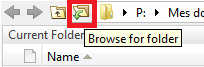
\includegraphics[width=80pt]{../../../img/matlabsimscape/matlab_01} dans le dossier dézippé jusqu'au dossier contenant les fichiers \og .slx \fg\ et \og Simscape \fg,\\
  \begin{center}
  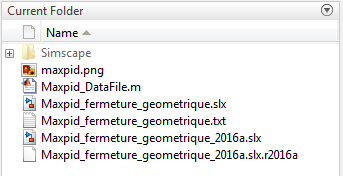
\includegraphics[width=0.3\linewidth]{../../../img/matlabsimscape/matlab_02}
  \end{center}
 \item Faire un clic-droit sur le dossier \og Simscape \fg\ et cliquer sur \og Add to Path \fg,\\
  \begin{center}
  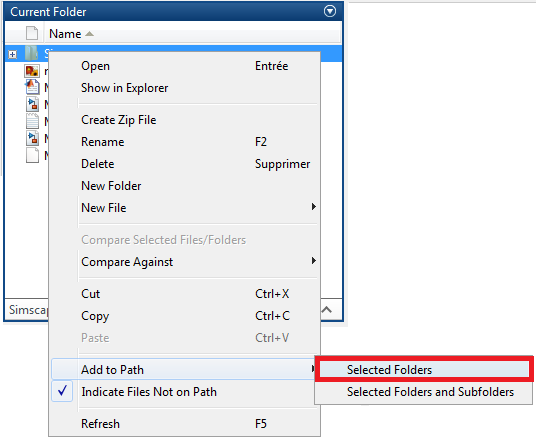
\includegraphics[width=0.4\linewidth]{../../../img/matlabsimscape/matlab_03}
  \end{center}
 \item Double-cliquer sur le fichier correspondant au TP et à la version de Matlab utilisée, il doit avoir une extension en \og slx \fg.\\
  \begin{center}
  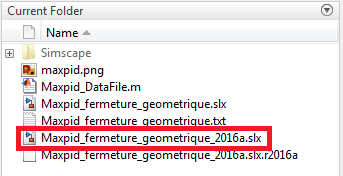
\includegraphics[width=0.4\linewidth]{../../../img/matlabsimscape/matlab_04}
  \end{center}
 \item Afin d'exporter des données, il est nécessaire d'insérer un bloc \textbf{To File} disponible dans la section \textit{Sinks} et de le connecter à la donnée à extraire,
 \item Double-cliquer dessus afin de modifier le paramètre \textit{Save format} en \textbf{Array}. Cela a pour effet de créer un fichier \textit{fichier.mat},
 \item Celui-ci peut être convertit en fichier \textit{fichier.csv} en utilisant les commandes suivantes:
 \texttt{FileData = load('fichier.mat');} \\
 \texttt{csvwrite('fichier.csv', FileData.ans);}
 \end{itemize}	

\label{proceduresimscape}
}

% Boîte d'exercice de maths pures, totalement décontextualisée du SI,
% pour les élèves n'ayant jamais fait de SI. S'utilise en complément
% de \aide (qui, elle, suppose déjà le contexte SI connu).
% Usage: \mathspure{texte}
\newcommand{\mathspure}[1]{%
\medskip\noindent\begin{tikzpicture}
\node[rounded corners=8,inner sep=8pt,fill=success!12,draw=success,line width=0.8pt] (box){%
\begin{minipage}{0.92\linewidth}
\textbf{\textcolor{success}{[M] Maths pures}} \\
\small #1
\end{minipage}
};
\end{tikzpicture}\medskip
}

\newcommand{\aidemecatroisd}{Une ressource permettant la prise en main du logiciel Meca3d est disponible \href{https://atemi.pagesperso-orange.fr/downloads/Meca3d/exemples/v18.0/Sinusmatic_v18.zip}{ici}}

% ------------------------------------------------------------------
% Blocs de différenciation par niveau (aides facultatives / bonus)
% ------------------------------------------------------------------

% Boîte de rappel / aide méthodologique facultative, destinée aux
% élèves qui ont besoin d'un coup de pouce. Usage: \aide{texte}
\newcommand{\aide}[1]{%
\medskip\noindent\begin{tikzpicture}
\node[rounded corners=8,inner sep=8pt,fill=info!12,draw=info,line width=0.8pt] (box){%
\begin{minipage}{0.92\linewidth}
\textbf{\textcolor{info}{[+] Aide / rappel}} \\
\small #1
\end{minipage}
};
\end{tikzpicture}\medskip
}

% Boîte de question bonus / approfondissement, facultative, destinée
% aux élèves les plus à l'aise. Usage: \bonus{texte}
\newcommand{\bonus}[1]{%
\medskip\noindent\begin{tikzpicture}
\node[rounded corners=8,inner sep=8pt,fill=warning!18,draw=warning,line width=0.8pt] (box){%
\begin{minipage}{0.92\linewidth}
\textbf{\textcolor{orange}{[++] Bonus / approfondissement}} \\
\small #1
\end{minipage}
};
\end{tikzpicture}\medskip
}

% Boîte de corrigé associée à une aide ou un bonus (fond neutre gris),
% à utiliser dans la partie \pagestyle{correction}. Usage: \corniveau{texte}
\newcommand{\corniveau}[1]{%
\medskip\noindent\begin{tikzpicture}
\node[rounded corners=8,inner sep=8pt,fill=gris25!15,draw=gris25,line width=0.8pt] (box){%
\begin{minipage}{0.92\linewidth}
\small #1
\end{minipage}
};
\end{tikzpicture}\medskip
}

% Légende à placer en tête de TP pour expliquer la convention [+] / [++]
% aux élèves. Usage: \legendeniveaux
\newcommand{\legendeniveaux}{%
\medskip\noindent\begin{tikzpicture}
\node[rounded corners=8,inner sep=8pt,fill=gris25!10,draw=gris25,line width=0.6pt] (box){%
\begin{minipage}{0.92\linewidth}
\footnotesize
\textbf{\textcolor{success}{[M] Maths pures}} : exercice de maths décontextualisé, pour s'entraîner sur le geste mathématique seul avant de l'appliquer au problème (utile si vous n'avez jamais fait de SI). \\
\textbf{\textcolor{info}{[+] Aide / rappel}} : rappel de cours ou méthode facultative, à utiliser si besoin (les élèves à l'aise peuvent l'ignorer). \\
\textbf{\textcolor{orange}{[++] Bonus}} : question d'approfondissement facultative, à traiter une fois le reste du sujet terminé.
\end{minipage}
};
\end{tikzpicture}\medskip
}





















% En tête et pied de page
\lhead{\nom}
\rhead{
\includegraphics[width=2cm]{../../../img/logo}}
\lfoot{\auteurs}
\cfoot{Page \thepage}

\fancypagestyle{correction}{%
  \fancyhf{}
  \lhead{\colorbox{danger}{\begin{minipage}{0.65\paperwidth} \textcolor{white}{\textbf{Correction}} \end{minipage}} }
  \rhead{
\includegraphics[width=2cm]{../../../img/logo}}
  \lfoot{Renaud Costadoat}
  \rfoot{\colorbox{danger}{\begin{minipage}{0.6\paperwidth} \begin{flushright}\textcolor{white}{\textbf{Correction}}\end{flushright} \end{minipage}} }}

\renewcommand{\footrulewidth}{0.4pt}

\usepackage{eso-pic}
\newcommand{\BackgroundPic}{%
\put(0,0){%
\parbox[b][\paperheight]{\paperwidth}{%
\vfill
\begin{center}
\hspace{0.5cm}\vspace{0.5cm}

\includegraphics[width=\paperwidth,height=\paperheight,%
keepaspectratio]{../../../img/fond3}%
\end{center}
\vfill
}}}

\newcommand{\BackgroundPicdeux}{%
\put(25,-30){%
\parbox[b][\paperheight]{\paperwidth}{%
\vfill
\begin{center}
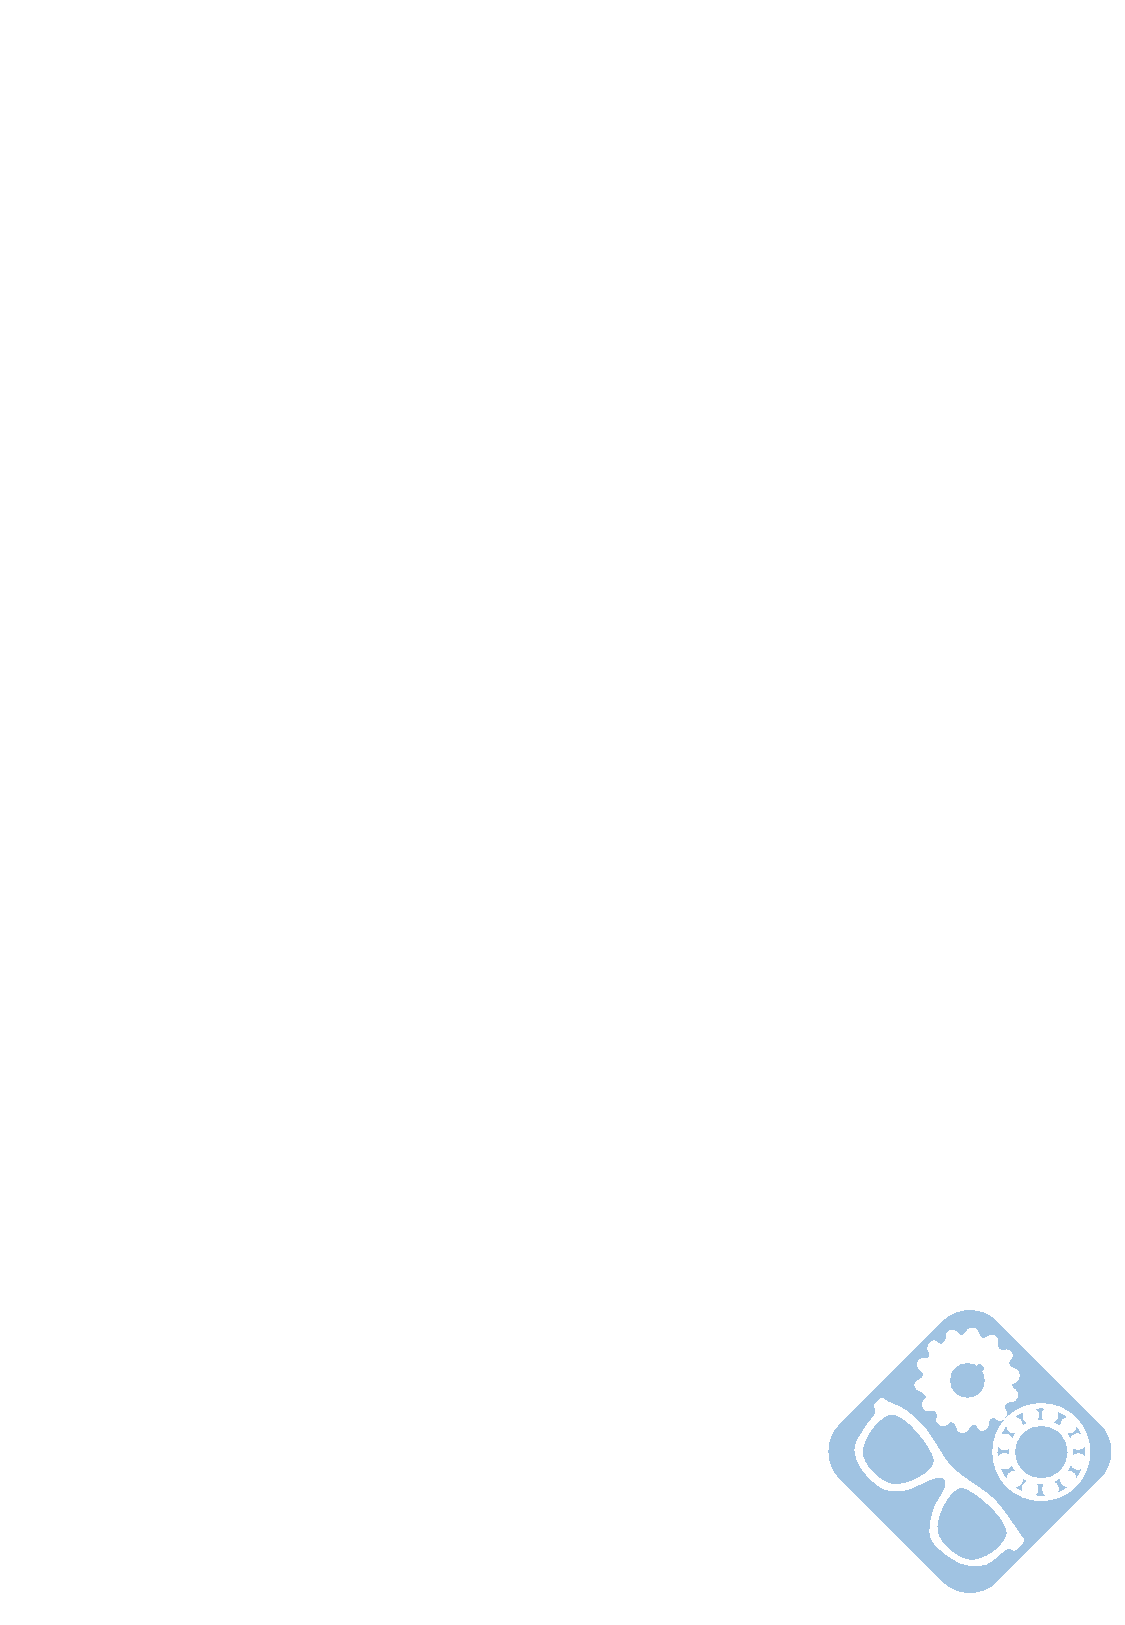
\includegraphics[width=\paperwidth,height=\paperheight,%
keepaspectratio]{../../../img/fond4}%
\end{center}
\vfill
}}}

\newcommand{\activite}[1]{\newpage \cleardoublepage
\renewcommand\arraystretch{2.5}\setcounter{section}{0}\setcounter{subsection}{0}
\ifthenelse{\equal{#1}{1}}{\begin{center}\begin{tabular}{|c|cc p{3cm}|}
\hline
\rowcolor{violt} \supportu & Act & Contenu & Compétences \\\hline
 \multirow{3}{*}{\includegraphics[width=0.2\linewidth]{\supportimageu}} & \begin{LARGE}\textbf{1}\end{LARGE} & \activiteun & \competenceun \\
 & \multicolumn{3}{l|}{Nom: .........................................................................}\\
 & \multicolumn{3}{l|}{Prénom: ....................................................................}\\\hline
\end{tabular}\end{center}}{}
\ifthenelse{\equal{#1}{2}}{\begin{center}\begin{tabular}{|c|cc p{3cm}|}
\hline
\end{tabular}\end{center}}{}}

\begin{document}

\pagestyle{empty}

\vspace*{-3\baselineskip}

\AddToShipoutPicture*{\BackgroundPic}

\ifdef{\auteurdeux}{\begin{tabular}{>{\columncolor{gray!00}}m{.33\linewidth} m{.27\linewidth} >{\columncolor{gray!00}}m{.3\linewidth}}
Séquence \sequence \ - \type \num \ - Îlot \numprint{\ilot} &  \multirow{3}{*}{\hspace{1cm}
\includegraphics[height=1.5cm]{../../../img/logo}} &  \begin{flushright} \multirow{4}{*}{\hspace{1cm}\includegraphics[height=4cm]{"img/qrcode"}}\end{flushright}\\
 \textbf{\institute} \\
 \auteurun\\
 \auteurdeux
\end{tabular}}{\begin{tabular}{>{\columncolor{gray!00}}m{.3\linewidth} m{.3\linewidth} >{\columncolor{gray!00}}m{.3\linewidth}}
Séquence \sequence \ - \type \num \ - Îlot \numprint{\ilot}  &  \multirow{3}{*}{\hspace{1cm}
\includegraphics[height=1.5cm]{../../../img/logo}} &  \begin{flushright} \multirow{4}{*}{\hspace{1cm}\includegraphics[height=4cm]{"img/qrcode"}}\end{flushright}\\
 \textbf{\institute} \\
 \auteurun
\end{tabular}}

\vspace{1cm}

\begin{center}\colorbox{white}{\huge{\nom}}\end{center}

\vspace{2cm}


\begin{center}\colorbox{white!20}{\includegraphics[height=5cm]{/home/renaud/Documents/Renaud/GitHub/django_education/django_education/static/systemes/\imageun}}\end{center}

\vspace{2cm}



\begin{tabular}{p{.15\linewidth} >{\columncolor{white}}p{.8\linewidth}}
    \rowcolor{gray!20}
    Référence & S\sequence \ - \type\num \ - I\numprint{\ilot} \\
    Compétences & \competences \\
 	\rowcolor{gray!20}
    Description & \descrip \\
    Système & \systemes
  \end{tabular}

\newpage

\AddToShipoutPicture{\BackgroundPicdeux}

\pagestyle{fancy}


\prob{Déterminer les caractéristiques d'un ressort.} 

\legendeniveaux

\section{Modèle du ressort élastique} 

Dans un premier temps, on considérera que le ressort utilisé dans cette expérience peut être modélisé comme un ressort élastique pur. 

\paragraph{Question 1:} Déterminer la raideur pure d'un ressort qui nécessite un effort de traction $F$ pour s'allonger d'une longueur $\Delta L$. On rappelle que la raideur d'un ressort s'exprime en $N.m^{-1}$.

\mathspure{Dans l'équation $F=K.\Delta L$, isolez $K$ en fonction de $F$ et $\Delta L$.}

\aide{la loi de Hooke relie la force exercée par un ressort élastique pur à son allongement par $F=K.\Delta L$. Isolez $K$ dans cette relation et vérifiez que l'unité obtenue est bien homogène à des $N.m^{-1}$.}

Une masse $m_1$ est suspendue à un ressort de raideur $K$, sa longueur mesurée est $L_1$. Une masse $m_2$ est suspendue à ce ressort (en remplacement de la précédente), sa longueur est maintenant $L_2$.

\paragraph{Question 2:} Déterminer la raideur de ce ressort en fonction de $L_1$, $L_2$, $m_1$ et $m_2$. Prendre toutes les hypothèses nécessaire à la mise en équation du problème. Est-ce que cela vous paraît raisonnable de prendre ces hypothèses ?

\mathspure{Soit le système à deux équations et deux inconnues $a$ et $b$ : $\begin{cases} y_1=a.x_1+b \\ y_2=a.x_2+b \end{cases}$. En soustrayant la deuxième équation à la première, l'inconnue $b$ disparaît. \textbf{Écrivez} l'équation obtenue après cette soustraction, puis \textbf{isolez} $a$ en fonction de $x_1$, $x_2$, $y_1$ et $y_2$.}

\aide{appliquez le principe fondamental de la statique (somme des forces nulle à l'équilibre) à chacune des deux masses. Vous obtenez un système de deux équations à deux inconnues : $K$ et $L_0$ (la longueur à vide du ressort, c'est-à-dire sans masse suspendue). Soustrayez les deux équations pour éliminer $L_0$ et isoler $K$.}

\bonus{à partir du système précédent, exprimez également $L_0$ en fonction de $L_1$, $L_2$, $m_1$ et $m_2$. Que représente physiquement cette grandeur, et comment pourriez-vous la vérifier expérimentalement de façon indépendante ?}

\section{Vérification de la raideur pure d'un ressort}

Il faudra pour la suite mettre en place un protocole de mesure permettant la répétabilité des mesures, il faut donc au préalable effectuer une installation propre et stable du matériel fournis. Il faudra aussi donner la liste et les caractéristiques (sensibilité, plage de mesure,...) du matériel de mesure utilisé.

\paragraph{Question 3:} Suspendre une masse $m_1$ à un ressort et mesurer sa longueur.

\paragraph{Question 4:} Suspendre une masse $m_2$ à un ressort et mesurer sa longueur.

\paragraph{Question 5:} Suspendre une masse $m_3$ à un ressort et mesurer sa longueur.

\subsection{Déterminer le comportement élastique d'un ressort}

\paragraph{Question 6:} A l'aide des résultats expérimentaux et des résultats de la question 2, déterminer la raideur $K$ du ressort.

\mathspure{Un élève mesure trois fois la même grandeur et trouve $5{,}1$ ; $5{,}4$ et $4{,}9$. Calculez la moyenne de ces trois valeurs (rappel : moyenne = somme des valeurs divisée par le nombre de valeurs).}

\aide{avec trois mesures $(m_1,L_1)$, $(m_2,L_2)$ et $(m_3,L_3)$, vous pouvez appliquer la formule de la question 2 à chaque couple de mesures possible (soit 3 valeurs de $K$), puis calculer la moyenne de ces valeurs. Quel est l'intérêt de moyenner plusieurs mesures plutôt que de n'en garder qu'une seule ?}

\section{Modèle du ressort élastique/amortisseur}  

Le modèle du ressort va maintenant évoluer afin de prendre en compte le coefficient d'amortissement du ressort. Pour cela, un fichier python  
\href{https://github.com/Costadoat/Sciences-Ingenieur/raw/master/S01\%20Analyse\%20fonctionnelle/TP01\%20Mod\%C3\%A9lisation\%20lin\%C3\%A9aire/Ilot_02\%20Ressort/modele_ressort_dyn.py}{\texttt{modele\_ressort\_dyn.py}} doit être ouvert avec le logiciel Spyder. Il permet de tracer le comportement d'un ressort amorti en fonction des paramètres suivants:
\begin{itemize}
 \item la durée de la mesure ($s$),
 \item la raideur du ressort ($N.m^{-1}$),
 \item la masse suspendue ($kg$),
 \item le coefficient d'amortissement ($N.m^{-1}.s$).
\end{itemize}

\paragraph{Question 7:} Définir l'influence de chacun de ces paramètres sur la courbe tracée.

\mathspure{Une fonction $f(t)$ est dite périodique de période $T$ si $f(t+T)=f(t)$ pour tout $t$. Sachant que $f$ a une période $T=4\,s$ et que $f(1)=3$, que vaut $f(5)$ ? Que vaut $f(9)$ ?}

\aide{sur une courbe oscillante amortie, on appelle \textbf{pseudo-période} la durée entre deux passages successifs par un même état (par exemple deux maximums consécutifs), et \textbf{amplitude} l'écart entre la position et sa valeur d'équilibre. Repérez ces deux grandeurs sur les courbes tracées par le script python.}

\bonus{l'équation différentielle du mouvement de la masse $m$ s'écrit $m.\ddot{x}(t)+f.\dot{x}(t)+K.x(t)=0$, où $f$ est le coefficient d'amortissement. En vous appuyant sur votre cours de mathématiques sur les équations différentielles du second ordre, exprimez le discriminant de l'équation caractéristique associée en fonction de $m$, $f$ et $K$, et donnez la condition sur ce discriminant pour observer un régime pseudo-périodique (oscillant amorti).}

\subsection{Mesure de la trajectoire amortie du ressort}

\paragraph{Question 8:} Filmer le mouvement du ressort après avoir lâché la masse (le ressort doit être en position de repos au départ).

\paragraph{Question 9:} Utiliser un logiciel de traitement pour déterminer la position de la masse en fonction du temps.

\subsection{Identifier le coefficient d'amortissement du ressort}

\paragraph{Question 10:} A partir des relevés expérimentaux et du programme python \\ \href{https://github.com/Costadoat/Sciences-Ingenieur/raw/master/S01\%20Analyse\%20fonctionnelle/TP01\%20Mesures\%20physiques/Ilot_02\%20Ressort/modele_ressort_dyn.py}{\texttt{modele\_ressort\_dyn.py}}, déterminer le coeffcient d'amortissement du ressort.

\aide{la démarche consiste à faire varier le coefficient d'amortissement dans le script python jusqu'à ce que la courbe simulée se superpose au mieux à votre courbe expérimentale (méthode dite "par recalage" ou "au jugé"). Vous connaissez déjà $K$ (question 6) et $m$ (masse suspendue), il ne reste donc qu'un seul paramètre inconnu à ajuster.}

\clearpage

\ifdef{\public}{\end{document}}{}

\newpage

\pagestyle{correction}

\section{Correction}

\paragraph{Question 1:}

\corniveau{\textbf{\textcolor{success}{[M] Maths pures :}} en divisant les deux membres de $F=K.\Delta L$ par $\Delta L$, on obtient $K=\dfrac{F}{\Delta L}$.}

\paragraph{Question 2:} 

$K=\frac{(m_1-m_2).g}{L_1-L_2}$, l'accélération de pesanteur est choisie égale à $9.81m.s^{-2}$.

\corniveau{\textbf{\textcolor{success}{[M] Maths pures :}} en soustrayant les deux équations, $y_1-y_2=a.(x_1-x_2)$ (le terme $b$ disparaît), soit $a=\dfrac{y_1-y_2}{x_1-x_2}$.}

\corniveau{\textbf{\textcolor{orange}{[++] Bonus :}} à l'équilibre, $m_1.g=K.(L_1-L_0)$ et $m_2.g=K.(L_2-L_0)$. En substituant l'expression de $K$ trouvée ci-dessus dans l'une des deux équations et en isolant $L_0$, on obtient $L_0=\dfrac{m_1.L_2-m_2.L_1}{m_1-m_2}$. Cette grandeur représente la longueur du ressort à vide (sans masse suspendue) ; elle peut être vérifiée expérimentalement en mesurant directement la longueur du ressort au repos, sans aucune masse accrochée.}

\paragraph{Question 6:}

\corniveau{\textbf{\textcolor{success}{[M] Maths pures :}} moyenne $=\dfrac{5{,}1+5{,}4+4{,}9}{3}=\dfrac{15{,}4}{3}\approx 5{,}13$.}

\paragraph{Question 7:}

\corniveau{\textbf{\textcolor{success}{[M] Maths pures :}} $f(5)=f(1+4)=f(1)=3$ et $f(9)=f(1+2\times 4)=f(1)=3$ : la fonction reprend la même valeur à chaque intervalle de $4\,s$.}

\corniveau{\textbf{\textcolor{orange}{[++] Bonus :}} l'équation caractéristique associée à $m.\ddot{x}(t)+f.\dot{x}(t)+K.x(t)=0$ est $m.r^2+f.r+K=0$, de discriminant $\Delta=f^2-4.m.K$. Le régime est pseudo-périodique (oscillant amorti) lorsque $\Delta<0$, c'est-à-dire lorsque l'amortissement $f$ est suffisamment faible devant $m$ et $K$.}

\end{document}
